\documentclass[10pt,a4paper,onecolumn]{article}
\usepackage{marginnote}
\usepackage{graphicx}
\usepackage{xcolor}
\usepackage{authblk,etoolbox}
\usepackage{titlesec}
\usepackage{calc}
\usepackage{tikz}
\usepackage{hyperref}
\hypersetup{colorlinks,breaklinks=true,
            urlcolor=[rgb]{0.0, 0.5, 1.0},
            linkcolor=[rgb]{0.0, 0.5, 1.0}}
\usepackage{caption}
\usepackage{tcolorbox}
\usepackage{amssymb,amsmath}
\usepackage{ifxetex,ifluatex}
\usepackage{seqsplit}
\usepackage{xstring}

\usepackage{float}
\let\origfigure\figure
\let\endorigfigure\endfigure
\renewenvironment{figure}[1][2] {
    \expandafter\origfigure\expandafter[H]
} {
    \endorigfigure
}


\usepackage{fixltx2e} % provides \textsubscript
\usepackage[
  backend=biber,
%  style=alphabetic,
%  citestyle=numeric
]{biblatex}
\bibliography{paper.bib}

% --- Splitting \texttt --------------------------------------------------

\let\textttOrig=\texttt
\def\texttt#1{\expandafter\textttOrig{\seqsplit{#1}}}
\renewcommand{\seqinsert}{\ifmmode
  \allowbreak
  \else\penalty6000\hspace{0pt plus 0.02em}\fi}


% --- Pandoc does not distinguish between links like [foo](bar) and
% --- [foo](foo) -- a simplistic Markdown model.  However, this is
% --- wrong:  in links like [foo](foo) the text is the url, and must
% --- be split correspondingly.
% --- Here we detect links \href{foo}{foo}, and also links starting
% --- with https://doi.org, and use path-like splitting (but not
% --- escaping!) with these links.
% --- Another vile thing pandoc does is the different escaping of
% --- foo and bar.  This may confound our detection.
% --- This problem we do not try to solve at present, with the exception
% --- of doi-like urls, which we detect correctly.


\makeatletter
\let\href@Orig=\href
\def\href@Urllike#1#2{\href@Orig{#1}{\begingroup
    \def\Url@String{#2}\Url@FormatString
    \endgroup}}
\def\href@Notdoi#1#2{\def\tempa{#1}\def\tempb{#2}%
  \ifx\tempa\tempb\relax\href@Urllike{#1}{#2}\else
  \href@Orig{#1}{#2}\fi}
\def\href#1#2{%
  \IfBeginWith{#1}{https://doi.org}%
  {\href@Urllike{#1}{#2}}{\href@Notdoi{#1}{#2}}}
\makeatother

% --- Page layout -------------------------------------------------------------
\usepackage[top=3.5cm, bottom=3cm, right=1.5cm, left=1.0cm,
            headheight=2.2cm, reversemp, includemp, marginparwidth=4.5cm]{geometry}

% --- Default font ------------------------------------------------------------
\renewcommand\familydefault{\sfdefault}

% --- Style -------------------------------------------------------------------
\renewcommand{\bibfont}{\small \sffamily}
\renewcommand{\captionfont}{\small\sffamily}
\renewcommand{\captionlabelfont}{\bfseries}

% --- Section/SubSection/SubSubSection ----------------------------------------
\titleformat{\section}
  {\normalfont\sffamily\Large\bfseries}
  {}{0pt}{}
\titleformat{\subsection}
  {\normalfont\sffamily\large\bfseries}
  {}{0pt}{}
\titleformat{\subsubsection}
  {\normalfont\sffamily\bfseries}
  {}{0pt}{}
\titleformat*{\paragraph}
  {\sffamily\normalsize}


% --- Header / Footer ---------------------------------------------------------
\usepackage{fancyhdr}
\pagestyle{fancy}
\fancyhf{}
%\renewcommand{\headrulewidth}{0.50pt}
\renewcommand{\headrulewidth}{0pt}
\fancyhead[L]{\hspace{-0.75cm}
\includegraphics[width=5.5cm]{logo.png}}
\fancyhead[C]{}
\fancyhead[R]{}
\renewcommand{\footrulewidth}{0.25pt}

\fancyfoot[L]{\parbox[t]{0.98\headwidth}{\footnotesize{\sffamily Adrian Danzglock,Vamsi Krishna Origanti, (). MujocoROS2Control:
Seamless MuJoCo Integration with ROS 2 for Robot Simulation and
Control. \textit{}, (), . \url{https://doi.org/}}}}


\fancyfoot[R]{\sffamily \thepage}
\makeatletter
\let\ps@plain\ps@fancy
\fancyheadoffset[L]{4.5cm}
\fancyfootoffset[L]{4.5cm}

% --- Macros ---------

\definecolor{linky}{rgb}{0.0, 0.5, 1.0}

\newtcolorbox{repobox}
   {colback=red, colframe=red!75!black,
     boxrule=0.5pt, arc=2pt, left=6pt, right=6pt, top=3pt, bottom=3pt}

\newcommand{\ExternalLink}{%
   \tikz[x=1.2ex, y=1.2ex, baseline=-0.05ex]{%
       \begin{scope}[x=1ex, y=1ex]
           \clip (-0.1,-0.1)
               --++ (-0, 1.2)
               --++ (0.6, 0)
               --++ (0, -0.6)
               --++ (0.6, 0)
               --++ (0, -1);
           \path[draw,
               line width = 0.5,
               rounded corners=0.5]
               (0,0) rectangle (1,1);
       \end{scope}
       \path[draw, line width = 0.5] (0.5, 0.5)
           -- (1, 1);
       \path[draw, line width = 0.5] (0.6, 1)
           -- (1, 1) -- (1, 0.6);
       }
   }

% --- Title / Authors ---------------------------------------------------------
% patch \maketitle so that it doesn't center
\patchcmd{\@maketitle}{center}{flushleft}{}{}
\patchcmd{\@maketitle}{center}{flushleft}{}{}
% patch \maketitle so that the font size for the title is normal
\patchcmd{\@maketitle}{\LARGE}{\LARGE\sffamily}{}{}
% patch the patch by authblk so that the author block is flush left
\def\maketitle{{%
  \renewenvironment{tabular}[2][]
    {\begin{flushleft}}
    {\end{flushleft}}
  \AB@maketitle}}
\makeatletter
\renewcommand\AB@affilsepx{ \protect\Affilfont}
%\renewcommand\AB@affilnote[1]{{\bfseries #1}\hspace{2pt}}
\renewcommand\AB@affilnote[1]{{\bfseries #1}\hspace{3pt}}
\renewcommand{\affil}[2][]%
   {\newaffiltrue\let\AB@blk@and\AB@pand
      \if\relax#1\relax\def\AB@note{\AB@thenote}\else\def\AB@note{#1}%
        \setcounter{Maxaffil}{0}\fi
        \begingroup
        \let\href=\href@Orig
        \let\texttt=\textttOrig
        \let\protect\@unexpandable@protect
        \def\thanks{\protect\thanks}\def\footnote{\protect\footnote}%
        \@temptokena=\expandafter{\AB@authors}%
        {\def\\{\protect\\\protect\Affilfont}\xdef\AB@temp{#2}}%
         \xdef\AB@authors{\the\@temptokena\AB@las\AB@au@str
         \protect\\[\affilsep]\protect\Affilfont\AB@temp}%
         \gdef\AB@las{}\gdef\AB@au@str{}%
        {\def\\{, \ignorespaces}\xdef\AB@temp{#2}}%
        \@temptokena=\expandafter{\AB@affillist}%
        \xdef\AB@affillist{\the\@temptokena \AB@affilsep
          \AB@affilnote{\AB@note}\protect\Affilfont\AB@temp}%
      \endgroup
       \let\AB@affilsep\AB@affilsepx
}
\makeatother
\renewcommand\Authfont{\sffamily\bfseries}
\renewcommand\Affilfont{\sffamily\small\mdseries}
\setlength{\affilsep}{1em}


\ifnum 0\ifxetex 1\fi\ifluatex 1\fi=0 % if pdftex
  \usepackage[T1]{fontenc}
  \usepackage[utf8]{inputenc}

\else % if luatex or xelatex
  \ifxetex
    \usepackage{mathspec}
    \usepackage{fontspec}

  \else
    \usepackage{fontspec}
  \fi
  \defaultfontfeatures{Ligatures=TeX,Scale=MatchLowercase}

\fi
% use upquote if available, for straight quotes in verbatim environments
\IfFileExists{upquote.sty}{\usepackage{upquote}}{}
% use microtype if available
\IfFileExists{microtype.sty}{%
\usepackage{microtype}
\UseMicrotypeSet[protrusion]{basicmath} % disable protrusion for tt fonts
}{}

\usepackage{hyperref}
\hypersetup{unicode=true,
            pdftitle={MujocoROS2Control: Seamless MuJoCo Integration with ROS 2 for Robot Simulation and Control},
            pdfborder={0 0 0},
            breaklinks=true}
\urlstyle{same}  % don't use monospace font for urls

% --- We redefined \texttt, but in sections and captions we want the
% --- old definition
\let\addcontentslineOrig=\addcontentsline
\def\addcontentsline#1#2#3{\bgroup
  \let\texttt=\textttOrig\addcontentslineOrig{#1}{#2}{#3}\egroup}
\let\markbothOrig\markboth
\def\markboth#1#2{\bgroup
  \let\texttt=\textttOrig\markbothOrig{#1}{#2}\egroup}
\let\markrightOrig\markright
\def\markright#1{\bgroup
  \let\texttt=\textttOrig\markrightOrig{#1}\egroup}


\usepackage{graphicx,grffile}
\makeatletter
\def\maxwidth{\ifdim\Gin@nat@width>\linewidth\linewidth\else\Gin@nat@width\fi}
\def\maxheight{\ifdim\Gin@nat@height>\textheight\textheight\else\Gin@nat@height\fi}
\makeatother
% Scale images if necessary, so that they will not overflow the page
% margins by default, and it is still possible to overwrite the defaults
% using explicit options in \includegraphics[width, height, ...]{}
\setkeys{Gin}{width=\maxwidth,height=\maxheight,keepaspectratio}
\IfFileExists{parskip.sty}{%
\usepackage{parskip}
}{% else
\setlength{\parindent}{0pt}
\setlength{\parskip}{6pt plus 2pt minus 1pt}
}
\setlength{\emergencystretch}{3em}  % prevent overfull lines
\providecommand{\tightlist}{%
  \setlength{\itemsep}{0pt}\setlength{\parskip}{0pt}}
\setcounter{secnumdepth}{0}
% Redefines (sub)paragraphs to behave more like sections
\ifx\paragraph\undefined\else
\let\oldparagraph\paragraph
\renewcommand{\paragraph}[1]{\oldparagraph{#1}\mbox{}}
\fi
\ifx\subparagraph\undefined\else
\let\oldsubparagraph\subparagraph
\renewcommand{\subparagraph}[1]{\oldsubparagraph{#1}\mbox{}}
\fi

\title{MujocoROS2Control: Seamless MuJoCo Integration with ROS 2 for
Robot Simulation and Control}

        \author[1]{Adrian Danzglock}
          \author[1]{Vamsi Krishna Origanti}
    
      \affil[1]{Robotics Innovation Center, German Research Center for
Artificial Intelligence (DFKI), Bremen, Germany}
  \date{\vspace{-7ex}}

\begin{document}
\maketitle

\marginpar{

  \begin{flushleft}
  %\hrule
  \sffamily\small

  {\bfseries DOI:} \href{https://doi.org/}{\color{linky}{}}

  \vspace{2mm}

  {\bfseries Software}
  \begin{itemize}
    \setlength\itemsep{0em}
    \item \href{https://github.com/openjournals/joss-reviews/issues/}{\color{linky}{Review}} \ExternalLink
    \item \href{}{\color{linky}{Repository}} \ExternalLink
    \item \href{}{\color{linky}{Archive}} \ExternalLink
  \end{itemize}

  \vspace{2mm}

  \par\noindent\hrulefill\par

  \vspace{2mm}

  {\bfseries Editor:} \href{}{} \ExternalLink \\
  \vspace{1mm}
    \vspace{2mm}

  {\bfseries Submitted:} \\
  {\bfseries Published:} 

  \vspace{2mm}
  {\bfseries License}\\
  Authors of papers retain copyright and release the work under a Creative Commons Attribution 4.0 International License (\href{http://creativecommons.org/licenses/by/4.0/}{\color{linky}{CC BY 4.0}}).

  
  \end{flushleft}
}

\hypertarget{summary}{%
\section{Summary}\label{summary}}

The \texttt{MujocoROS2Control} hardware interface enables seamless
integration between MuJoCo (Todorov, Erez, and Tassa 2012), a
high-performance physics engine, and ROS 2 (ROS-Controls Team 2024a), a
widely adopted middleware for robotic systems. This interface provides
an efficient solution for simulating and controlling robots using
MuJoCo's physics capabilities within the ROS 2 ecosystem.

To support ROS-based workflows, we developed a dedicated URDF-to-MJCF
conversion script. This tool translates URDF models into MJCF (MuJoCo
XML format), preserving kinematic and dynamic properties and allowing
custom MuJoCo-specific parameters such as sensors, actuators, and
collision definitions to be specified directly in the URDF. This
conversion ensures compatibility and adaptability for simulation.

\texttt{MujocoROS2Control} bridges the gap between ROS 2 and MuJoCo,
offering a streamlined workflow for simulation, controller testing, and
reinforcement learning.

\hypertarget{statement-of-need}{%
\section{Statement of Need}\label{statement-of-need}}

Developing and validating control algorithms for robotic systems often
requires extensive testing, which on physical hardware can be expensive,
time-consuming, and subject to wear. Accurate simulation environments
are essential for safe and scalable development.

MuJoCo (Multi-Joint dynamics with Contact) is a fast and accurate
physics engine designed for robotics, control, biomechanics, and
reinforcement learning. It provides: - Precise multi-body dynamics with
advanced numerical integration, - High-speed simulation for real-time
control and machine learning, - Sophisticated contact modeling and soft
constraint handling, - Flexible actuator models and comprehensive sensor
support.

Despite these capabilities, MuJoCo lacks native support for ROS 2,
limiting its adoption in modern robotic development pipelines.
\texttt{MujocoROS2Control} addresses this gap, enabling users to
simulate ROS 2-compatible robots in MuJoCo with minimal overhead.

Our framework has been successfully used to test components such as
force-torque sensor gravity compensation, torque-based Cartesian
controllers, and Dynamic Movement Primitives (DMP)-based skill
reproduction (Fabisch 2024).

\hypertarget{implementation}{%
\section{Implementation}\label{implementation}}

\texttt{MujocoROS2Control} integrates MuJoCo with the
\texttt{ros2\_control} framework. A key component is the URDF-to-MJCF
converter, which maintains fixed joints (which MuJoCo typically
collapses), allows sensor and actuator tags within URDFs, and generates
MJCF files compatible with MuJoCo's expectations.

The interface supports: - Direct torque control, - PID-based
position/velocity/acceleration control, - MuJoCo's native actuator
models.

Joint states and simulation time are published for synchronization with
the ROS 2 system time (\texttt{/clock}). Sensors defined in the URDF
(force-torque, IMU, pose, RGB-D camera) are exposed as individual ROS
nodes using \texttt{realtime\_tools} (ROS-Controls Team 2024b) to
maintain real-time performance.

\hypertarget{examples}{%
\section{Examples}\label{examples}}

\hypertarget{franka-fr3-with-industrealkit-gears}{%
\subsection{Franka FR3 with IndustRealKit
Gears}\label{franka-fr3-with-industrealkit-gears}}

This example integrates the Franka FR3 robot (FRANKA ROBOTICS 2024) with
high-resolution gear models from the IndustRealKit (Tang et al. 2023).
MuJoCo actuators are used to generate joint torques, although the
implemented PID control and torque control are also supported. For the
high-resolution collision modeling, we use CoaCD (Wei et al. 2022) to
create multiple convex hulls from complex mesh geometry. The
URDF-to-MJCF converter automatically replaces original mesh files in the
mjcf, when the converted files are in the same directory.

\begin{figure}
\centering
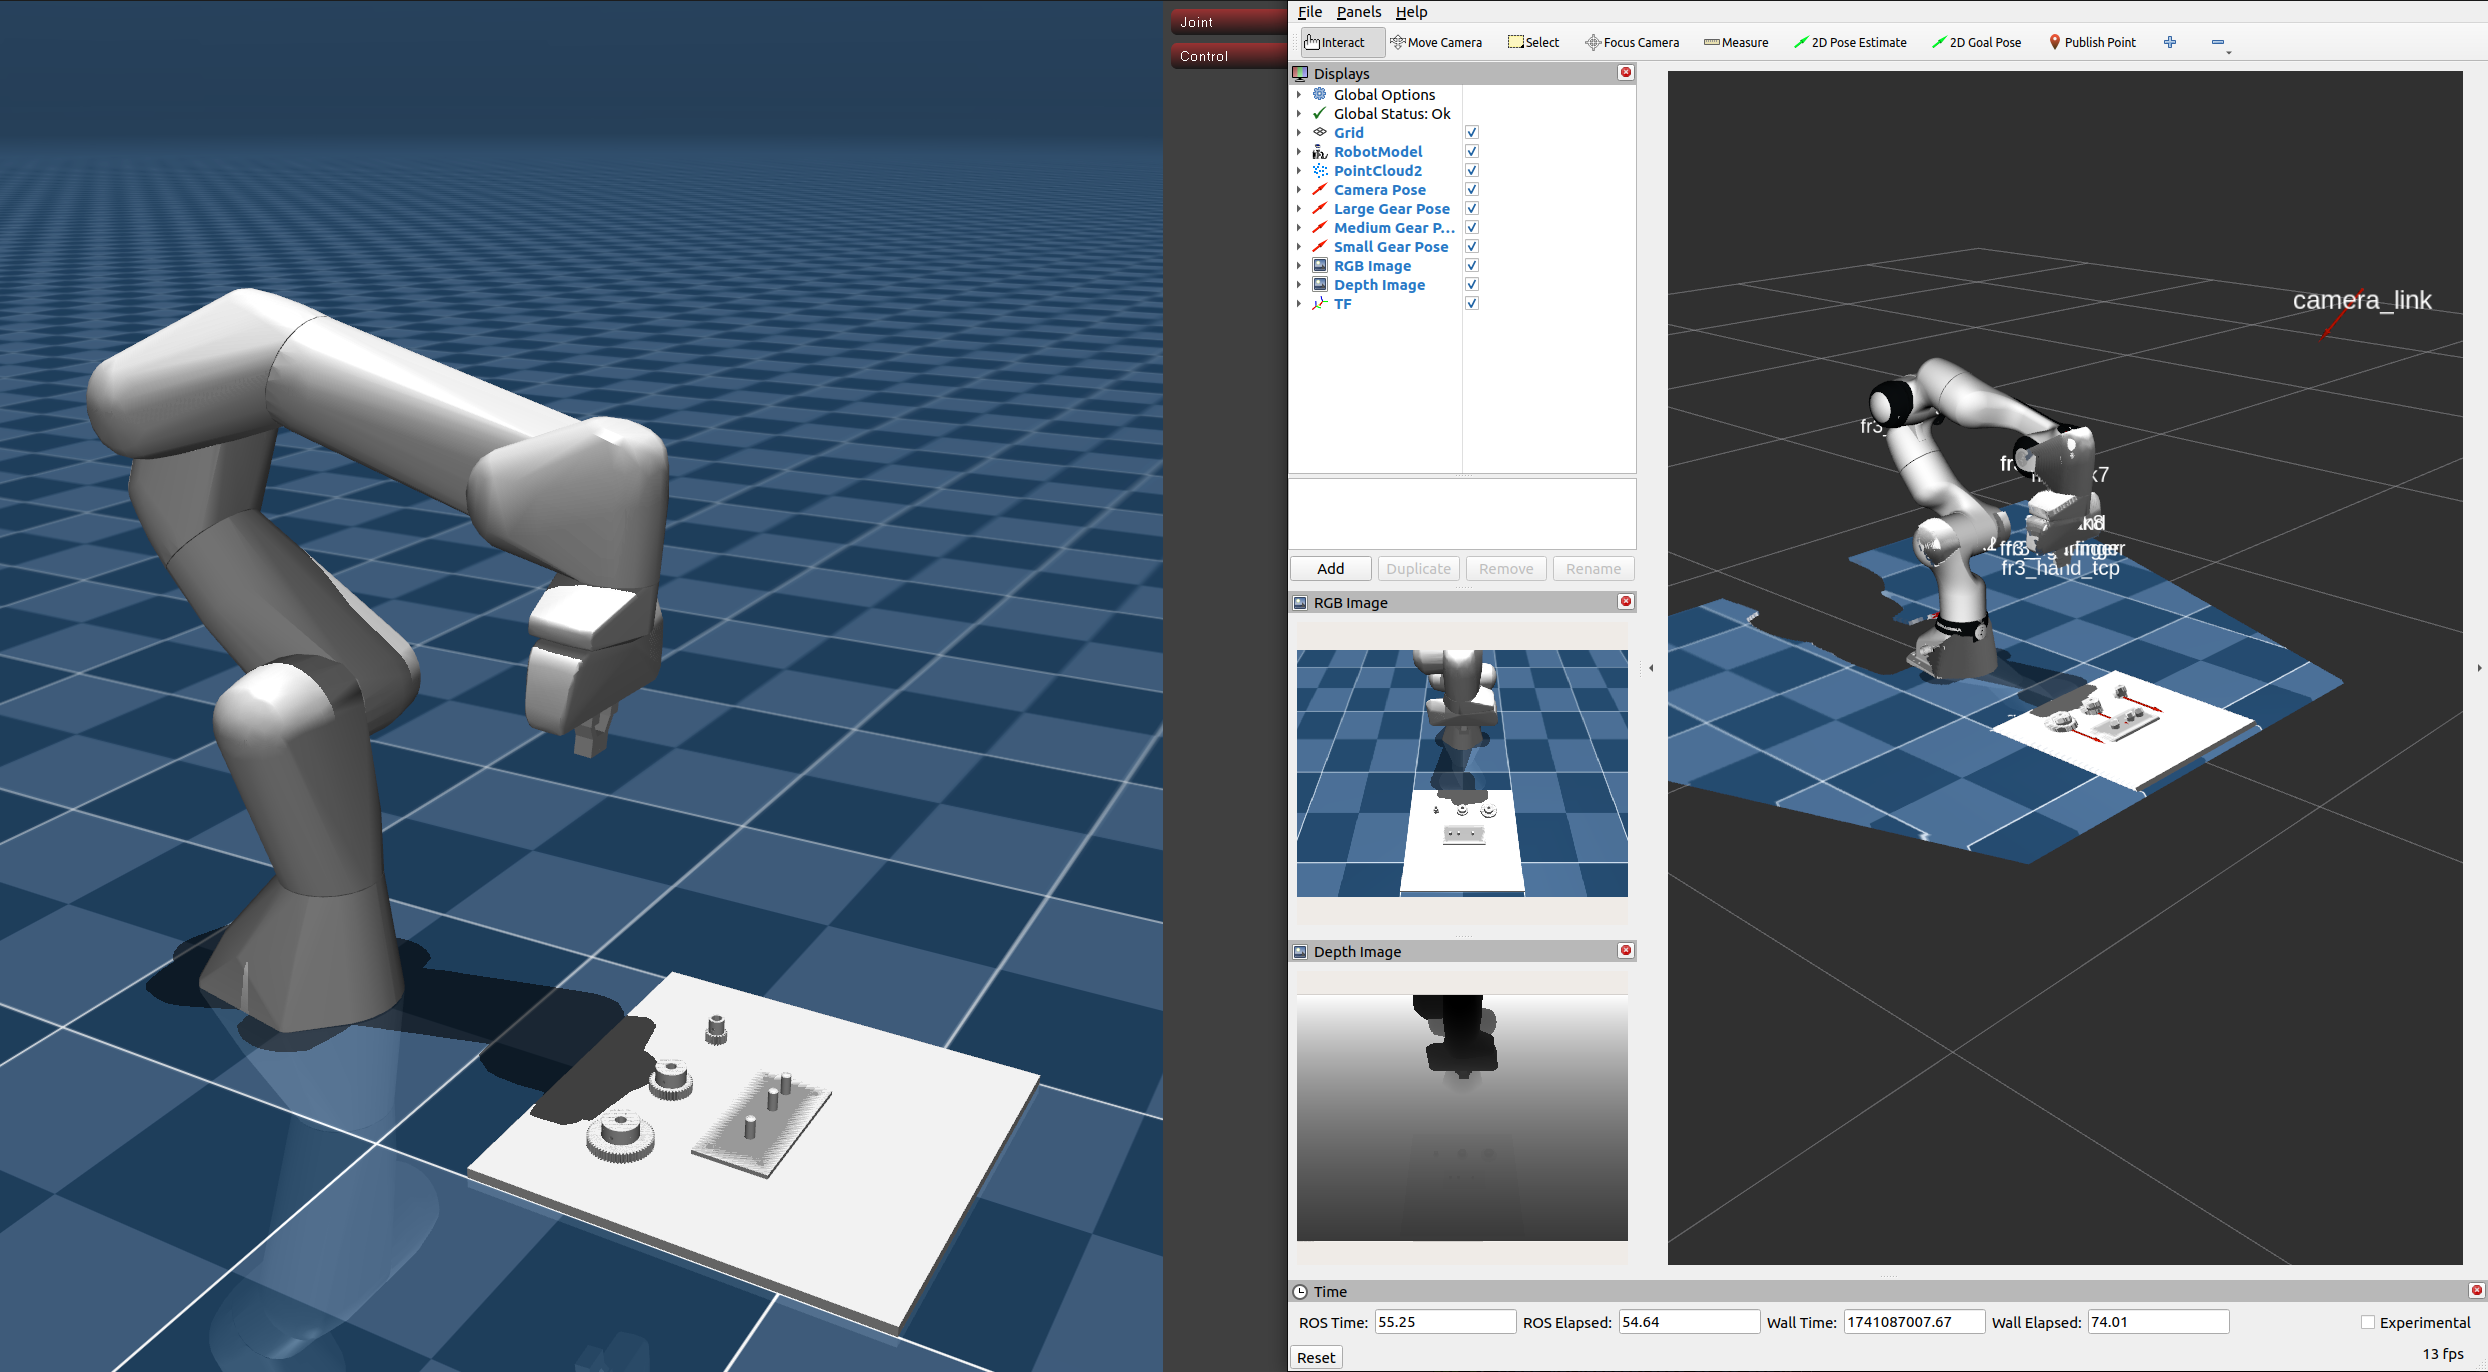
\includegraphics{./figures/franka_rgbd_example.png}
\caption{Franka FR3 controlled with ROS 2 Joint Trajectory Controller}
\end{figure}

\hypertarget{imrk-system}{%
\subsection{IMRK System}\label{imrk-system}}

In this example, we simulate the iMRK system developed at DFKI Bremen,
consisting of two KUKA LBR iiwa 14 robots ({\textbf{???}}). A ROS2
Cartesian impedance controller (migrated version of (Mayr and
Salt-Ducaju 2024)) is used for each arm. MuJoCo actuators manage the
Robotiq 2F grippers, and force-torque sensors are simulated at both
end-effectors.

\begin{figure}
\centering
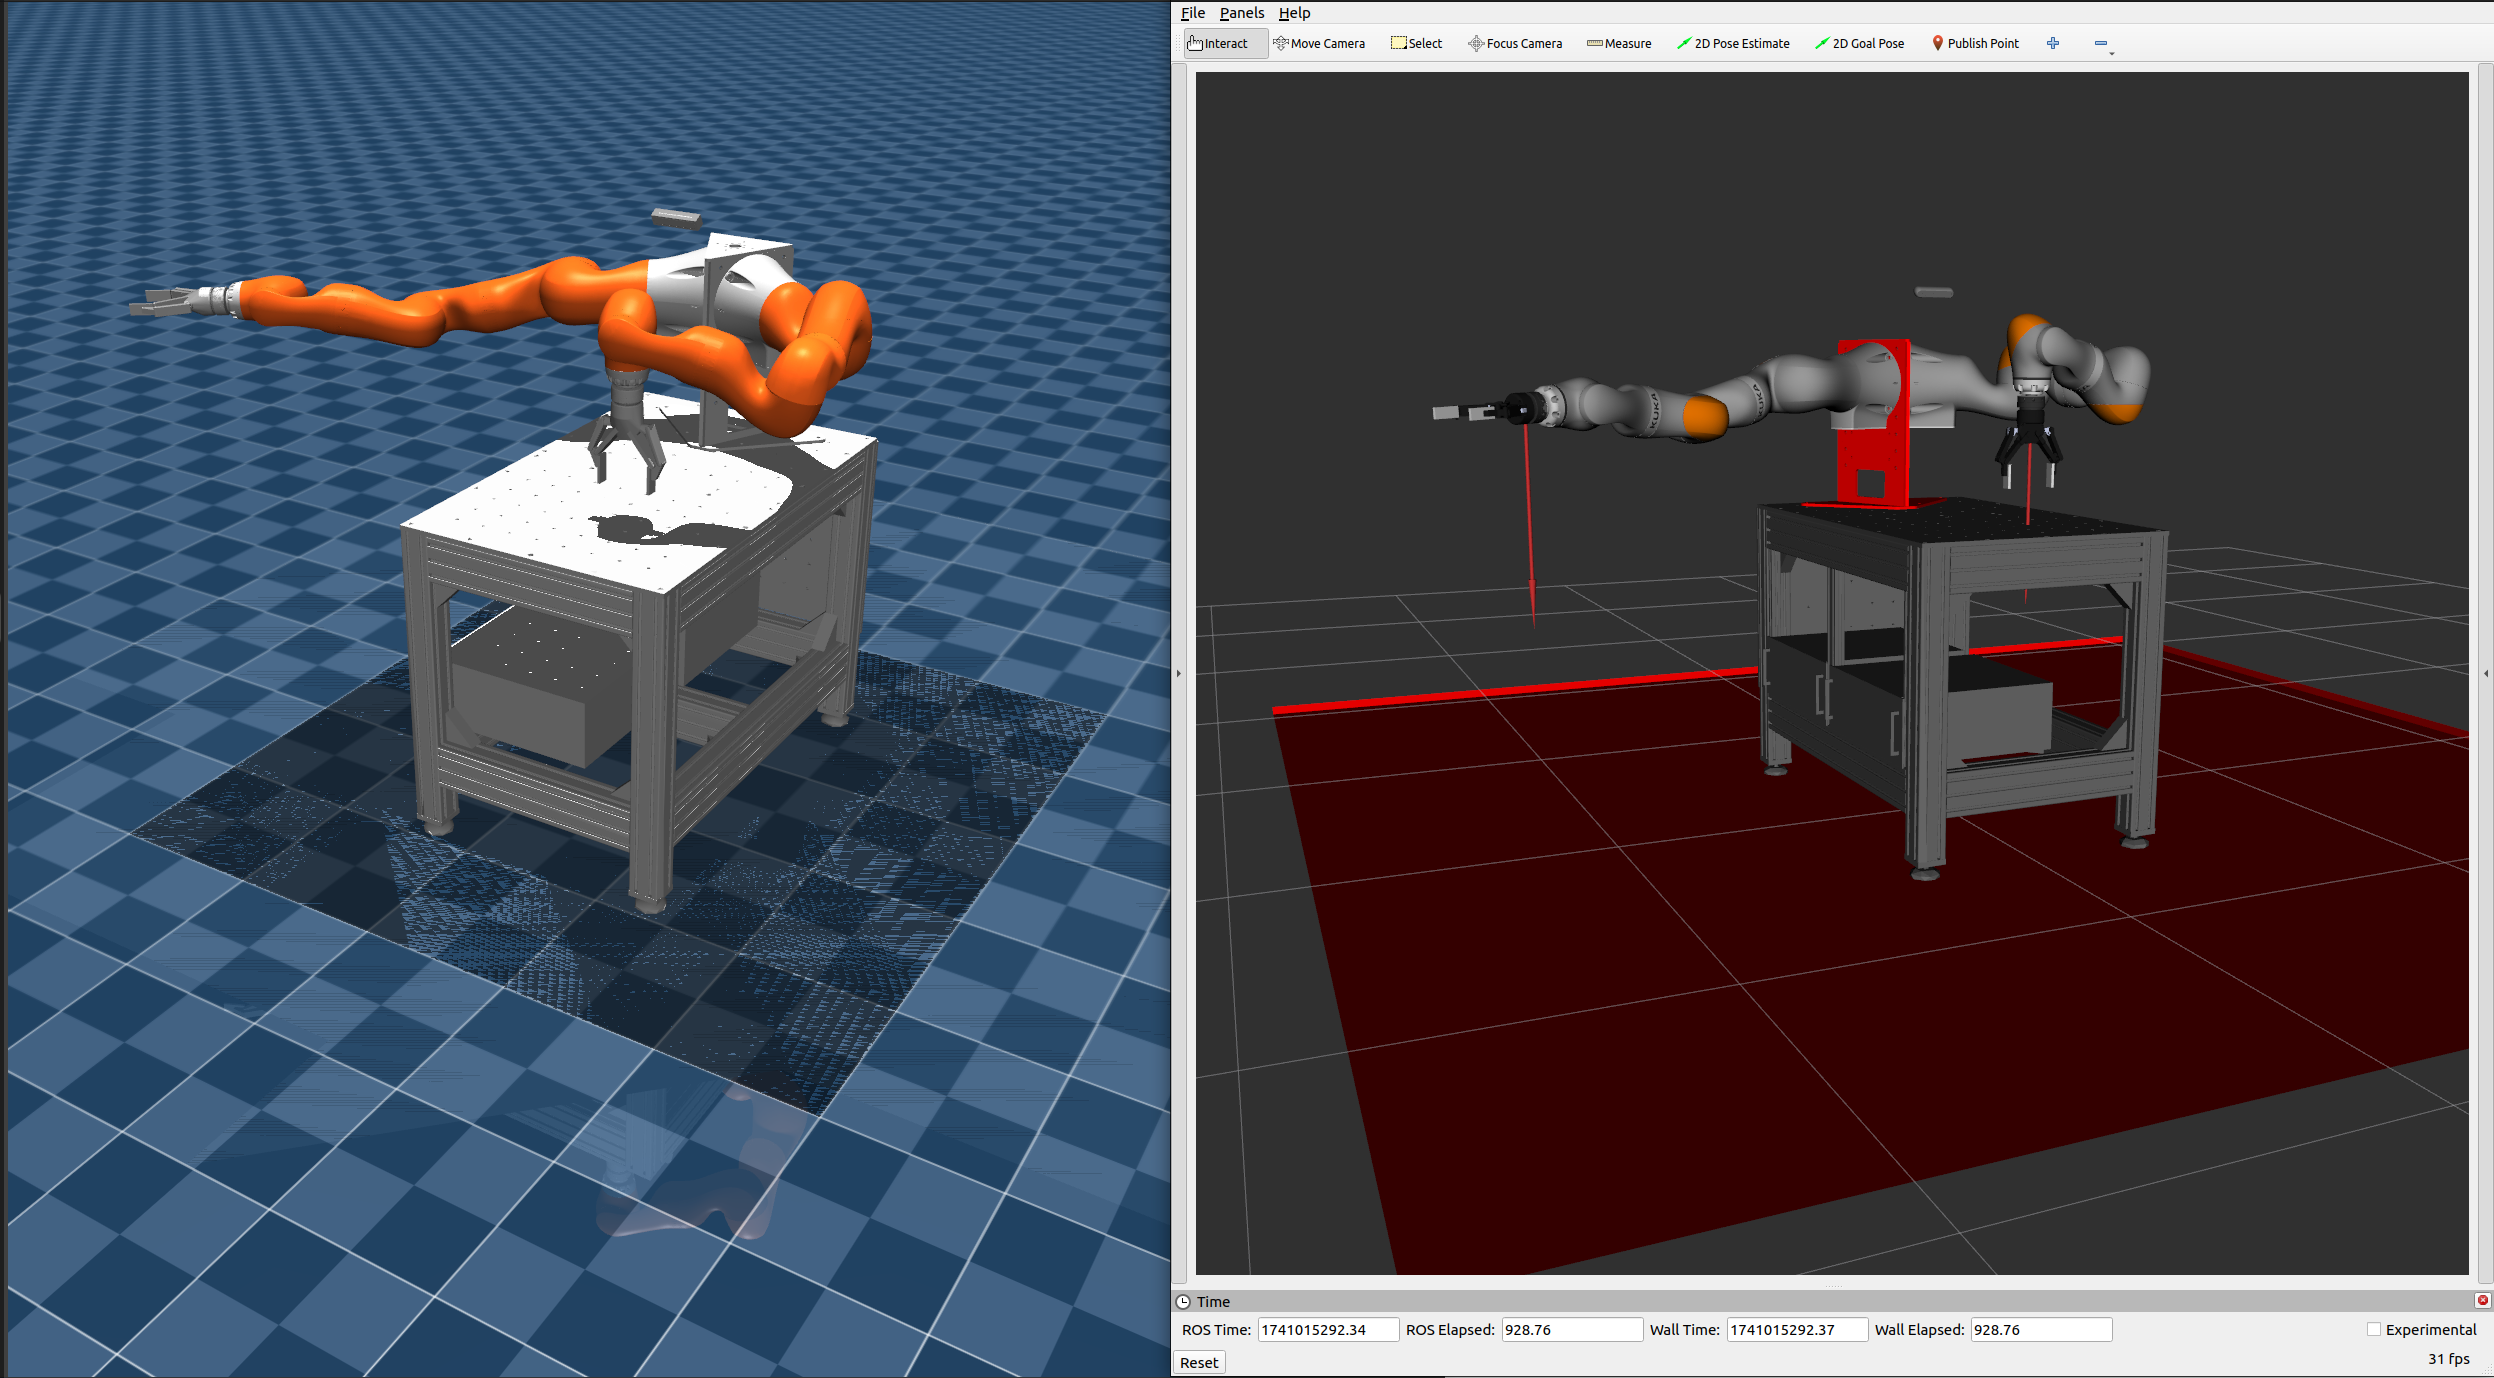
\includegraphics{./figures/kuka_imrk_example.png}
\caption{IMRK with Robotiq 2F Gripper and Robotiq FT300 Sensor}
\end{figure}

(Note: The IMRK robot description is internal and not included in the
public examples.)

\hypertarget{conclusion}{%
\section{Conclusion}\label{conclusion}}

\texttt{MujocoROS2Control} enables high-fidelity robotic simulation by
integrating MuJoCo with ROS 2. Through its robust conversion utilities,
sensor bridging, and actuator support, it provides a reliable framework
for control development, validation, and machine learning research.

Its lightweight design and fast simulation performance make it
well-suited for force-based control, trajectory optimization, and
reinforcement learning applications. Future enhancements may include
support for additional sensor types, multi-robot coordination, and
real-time closed-loop learning.

\hypertarget{acknowledgements}{%
\section{Acknowledgements}\label{acknowledgements}}

This library was initiated and developed at the Robotics Innovation
Center, German Research Center for Artificial Intelligence (DFKI GmbH),
Bremen, Germany, as part of the HARTU Project. This project received
funding from the European Union's Horizon Europe research and innovation
program under grant agreement No.~101092100.

\hypertarget{references}{%
\section*{References}\label{references}}
\addcontentsline{toc}{section}{References}

\hypertarget{refs}{}
\begin{cslreferences}
\leavevmode\hypertarget{ref-Fabisch2024}{}%
Fabisch, Alexander. 2024. \emph{Journal of Open Source Software} 9 (97):
6695. \url{https://doi.org/10.21105/joss.06695}.

\leavevmode\hypertarget{ref-franka_description}{}%
FRANKA ROBOTICS. 2024.
\url{https://github.com/frankaemika/franka_description}.

\leavevmode\hypertarget{ref-mayr2024cartesian}{}%
Mayr, Matthias, and Julian M. Salt-Ducaju. 2024. ``A C++ Implementation
of a Cartesian Impedance Controller for Robotic Manipulators.''
\emph{Journal of Open Source Software} 9 (93): 5194.
\url{https://doi.org/10.21105/joss.05194}.

\leavevmode\hypertarget{ref-ros2_control}{}%
ROS-Controls Team. 2024a.
\url{https://github.com/ros-controls/ros2_control}.

\leavevmode\hypertarget{ref-realtime_tools}{}%
---------. 2024b. \url{https://github.com/ros-controls/realtime_tools}.

\leavevmode\hypertarget{ref-tang2023industreal}{}%
Tang, Bingjie, Michael A Lin, Iretiayo Akinola, Ankur Handa, Gaurav S
Sukhatme, Fabio Ramos, Dieter Fox, and Yashraj Narang. 2023.
``IndustReal: Transferring Contact-Rich Assembly Tasks from Simulation
to Reality.'' In \emph{Robotics: Science and Systems}.

\leavevmode\hypertarget{ref-todorov2012mujoco}{}%
Todorov, Emanuel, Tom Erez, and Yuval Tassa. 2012. ``MuJoCo: A Physics
Engine for Model-Based Control.'' In \emph{2012 Ieee/Rsj International
Conference on Intelligent Robots and Systems}, 5026--33. IEEE.
\url{https://doi.org/10.1109/IROS.2012.6386109}.

\leavevmode\hypertarget{ref-wei2022coacd}{}%
Wei, Xinyue, Minghua Liu, Zhan Ling, and Hao Su. 2022. ``Approximate
Convex Decomposition for 3d Meshes with Collision-Aware Concavity and
Tree Search.'' \emph{ACM Transactions on Graphics (TOG)} 41 (4): 1--18.
\end{cslreferences}

\end{document}